%----------------------------------------
% Write your notes here
%----------------------------------------

\section{Introduction}
This is an overview of Sid's lecture for Modeling Social Data. These notes will cover three main topics:
\begin{enumerate}
  \item Computational Tractability
  \item Asymptotic Order of Growth (Big O)
  \item Common Running Times
  	\begin{itemize}
  		\item Data Structures
  		\item Algorithms
	\end{itemize}
\end{enumerate}

In general, when we are analyzing algorithms, we want to think about the worst-case, average-case, and amortized run time of them.

\section{Definitions}


Let us start with the concept of Big O notation and define the upper bound. $T(n)$, the running time, is $\textit{O}(t(n))$ if there exists a $c >$ 0, $n_{0} \geq$ 0 such that $T(n) \leq c\cdot t(n)$ for all $n > n_{0}$. Here is an example. Suppose $T(n) = 32n^{2} + 17 \cdot n +1$. Therefore, $T(n) = O(n^{2})$ for $ c=50, n_{0} =1$. \\

The lower bound is the following.  $T(n)$ is $\Omega(t(n))$ if there exists a $c >$ 0, $n_{0} \geq$ 0 such that $T(n) \geq c\cdot t(n)$ for all $n > n_{0}$. Using the same $T(n)$ as defined in the upper bound example, we get $T(n) = \Omega(n^{2})$ for $ c=31, n_{0} \geq 1$. \\


The tight bound is defined as follows. $c_{1} \cdot t(n) \leq T(n) \leq c_{2} \cdot t(n)$ for all n $>$ $n_{0} =1$ such that $T(n) = \Theta (T(n))$. Using the same T(n) as defined in the upper bound example, we get $T(n) = \Theta(n^{2})$. \\

\section{Rules of Thumb}

\begin{enumerate}
  \item If $T(n)  = a_{0} + a_{1}n + a_{2}n^{2} + ... + a_{d}n^{d}$, then T(n) = $\Theta (n^{d})$.
  \item $O(\log_a n) = O(\log_a n)$. Doesn't matter what base is.
  \item For every $r>1$ and $d>0$, $n^{d} = O(r^{n})$. Exponential function will always be dominated by a polynomial. This is true for big $n$, not necessarily for small $n$.
\end{enumerate}

\section{Examples}


\begin{enumerate}
  \item $O(n)$. An example of algorithm that runs linear time is computing the max of $n$ numbers. The algorithm would set initialize the maximum at 0 and then iterate through the set, and compare each value $i$ to the maximum. If the value $i$ is greater than the max value, the max value would become $i$. We assume computer computation is $O(1)$. In reality, the real amount of time depends on the bits sent. Because the set has length n, there are $n \cdot O(1) = O(n)$ comparisons and as such runs in linear time
  
  \item Divide and conquer algorithms such as sorting have $O(n \cdot log (n))$ time. There are $log (n)$ levels since the amount doubles every time, and on each level it takes $O(n)$ time to sort. $\Omega(n \cdot log n)$ is much harder to determine, as it is much more difficult to come up with a hypothetical lower bound as one needs to show there is no possible computational model that is higher than the proposed lower bound.  
  
  \item Bubblesort has quadratic time, $O(n^{2})$. This is because their are $n \cdot O(n)$ = $O(n^{2})$, where there are n items in the array and a linear scan of the array takes $O(n)$ (from example 1). 
  
   \item Quicksort has an expected run time of $O(n \cdot log (n))$ if the picks are pretty good, which they are on average. The worst case time for quick sort  $O(n^{2})$.
   
   \item $O(n^{3})$ often comes up in graphs. Specifically, if you are trying to count triangles in a graph, it would take cubic time. You would think that matrix multiplication is $O(n^{3})$, but in actuality the fastest running time is something like $O(n^{2.37})$. 
   
   \item $O(log(n))$ is even better than linear time. Each iterations halves the amount of array, so it reduces in size exponentially, and as such takes $O(log(n))$.
  
\end{enumerate}

\section{Binary Trees}

Trees are useful because they allow you to find things quickly. 

\Tree [.4 [ 1 3 ] .2 [ 5 7 ] .6   ] \\

As we can see, it much quicker to find a number in a tree then it is linearly since linear search has n time which is bad. 

\section{Hash Tables}





A hash table is a data structure that maps keys to values. Here is an illustration: \\

\begin{tikzpicture}

\draw[step=0.5cm,color=gray] (0,0) grid (.5,.5);
\node at (.25,.25) {h};
\node at (1.5,.25) { $h(x)$ \vspace{2cm} $\longrightarrow$};

\node at (-.5,.25) {$\longrightarrow$};
\node at (-1.0,.25) {k};



\draw[step=0.5cm,color=gray] (2.4999,-1) grid (3.0,1.50);

\end{tikzpicture}

The hash is h, and the function $h(x)$ defines which bin to put each item. This is done so as to minimize the length of each bucket in the hash. A hash table has $O(1)$ access, which is a big increase over using a tree for searching. \\

Now let's think about the chance that 2 items $k_{1}, k_{2}$ collide in the same bin, represented by: 

\begin{tikzpicture}

\draw[step=0.5cm,color=gray] (0,0) grid (.5,.5);
\node at (.25,.25) {h};
\node at (1.5,.25) { $h(x)$ \vspace{2cm} $\longrightarrow$};
\node at (-1.25,.25) {$k_{1},k_{2}$};
\node at (-.5,.25) {$\longrightarrow$};


\draw[step=0.5cm,color=gray] (2.4999,-1) grid (3.0,1.50);
\node at (4.0,0.75) {$\longrightarrow k_{1},k_{2}$ };

\end{tikzpicture}

Here, $k_{1},k_{2}$ is a linked list for the second from the top bin. This function is deterministic, so for the same input, the function will spit out the same output. Now, how long will the linked list get? On average,there should be a constant since the hash function should spread this out. The probability of a collision is $P(colllision) = \frac{1}{n}$. The expected number of collisions therefore is ${n \choose c} \cdot \frac{1}{n}$ = $\frac{O(n)}{n}$ = $O(n) \cdot$ items per bin. \\

What size hash table should we want? We only want the hash table to be slightly bigger than $n$, as that will have a pretty good distribution. This is an application of the balls and bins problem. The running time of this is $\Theta(\frac{lg(n)}{lg(lg(n)))}$.

\section{Application to Joining Data}

We will now take all that we have learned and apply it to gain a better understanding of the running time associated with joining data. Suppose we have 2 tables and want to combine them: \\

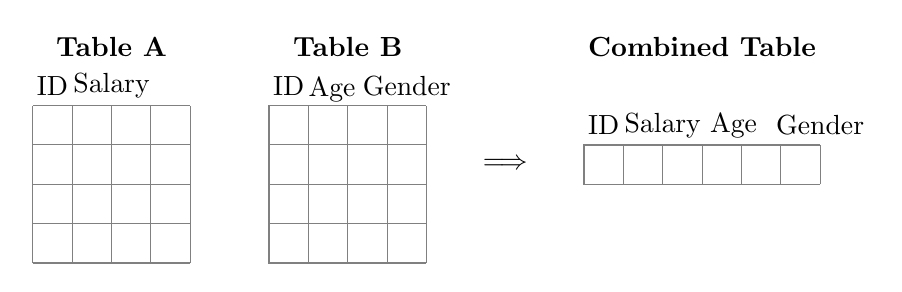
\begin{tikzpicture}

\draw[step=0.5cm,color=gray] (-1,-1) grid (1,1);
\node at (0,1.75) {\textbf{Table A}};

\node at (-.75,1.25) {ID};
\node at (0,1.25) {Salary};

\draw[step=0.5cm,color=gray] (1.99,-1) grid (4,1);
\node at (3,1.75) {\textbf{Table B}};

\node at (2.25,1.25) {ID};
\node at (2.8,1.20) {Age};
\node at (3.75,1.25) {Gender};
\node at (5,.25) {$\Longrightarrow$}; 

\draw[step=0.5cm,color=gray] (5.99,0) grid (9,.5);
\node at (7.5,1.75) {\textbf{Combined Table}};
\node at (6.25,.75) {ID};
\node at (7.0,.75) {Salary};
\node at (7.9,.75) {Age};
\node at (9.0,.75) {Gender};

\end{tikzpicture} \\

The tables are of size $n\times{k}$. The first column of each table corresponds to the ID, the others correspond to different features. Table A and Table B have different features; for example, Table A might have data on Salary while Table B might have data on age and gender (as shown above). The question is, how do you combine these tables into one table which has all the features corresponding to the same ID? \\

If you naively search both columns in a linear scan, the running time is $O(n^{2})$. But how could we do better? We could use a binary tree to create an index. It would take log time to find index through tree, and for n rows, the running time would be $O(n \cdot log(n)) $ which is an improvement. If we want to move from log to constant time, we'll have to use hashing: \\

\begin{tikzpicture}

\draw[step=0.5cm,color=gray] (0,0) grid (.5,.5);
\node at (.25,.25) {h};
\node at (1.5,.25) { $h(x)$ \vspace{2cm} $\longrightarrow$};

\node at (-.5,.25) {$\longrightarrow$};
\node at (-1.0,.25) {k};

\draw[step=0.5cm,color=gray] (2.4999,-1) grid (3.0,1.50);

\end{tikzpicture}

Here, our k will be the rows and our buckets will be rows of the combined table. How long will it take to make this table? Each operation takes constant time, so this is linear and as such runs in $O(n)$ time. You put rows from Table B into the hash, and where there is a collision, the ID is both in Table A and B. This works because the hash table is deterministic, and the features that correspond to the same ID for each table will be sent by the hash function to the same bucket. It wouldn't work if the hash function places rows in a table randomly. 

\section{Conclusion}

This was a high level overview of data structures and algorithms. For some parting wisdom, Sid mentioned that if you connect the person who discovered the algorithm to the algorithm itself it makes studying them that much more exciting. After Sid's lecture, Hoffman introduced us to the R programming language. 
